\section{Menu}
The user interface is based on a menu system where the user can navigate using a keypad. The menu system is implemented as a state machine. This is done by using two different switch statements. The first is \mintinline{c}{KeyInput} which calls the function corresponding to the current \mintinline{c}{menuState} the menu is in. The state function are updating the \mintinline{c}{menuState} depending on the input from the user. 
It is changed to the state corresponding to the selected part of the menu.

\begin{lstlisting}[caption={The statemachine of menu system.}, label={lst:menu}, language=C,directivestyle={\color{black}},
emph={int,char,double,float,unsigned},emphstyle={\color{blue}}]
void KeyInput(void)
{
	switch(menuState)
	{
		case 0:
			state00();
			break;
		case 1:
			state01();
			break;
		case 2:
			state02();
			break;
		case 3:
			state03();
			break;
		case 4:
			state04();
			break;
		case 5:
			state05();
			break;
		case 6:
			state06();
			break;
	}
	// reset global variable so that we know the input is dealt with
	_delay_ms(10);
	keyPushInput = KEY_NULL;
}
\end{lstlisting}
\vspace{10pt}
The \mintinline{c}{menuState} functions are responsibly for the action of that \mintinline{c}{menuState}. This could be showing new information on the screen or running the ADC and outputting the result.
\newpage
\begin{lstlisting}[caption={Implementation of the states in the menu system.}, label={lst:menustate}, language=C,directivestyle={\color{black}},
emph={int,char,double,float,unsigned},emphstyle={\color{blue}}]
// Start count
void state00(void)
{
	switch(keyPushInput)
	{
		case KEY_UP: // Change to state04
			menuState = 3;
			LCDChange = 1;
			menuState03Func();
			break;
		case KEY_DOWN: // Change to state02
			menuState = 3;
			LCDChange = 1;
			menuState03Func();
			break;
		case KEY_STAR: // Do nothing
			break;
		case KEY_SQUARE: // Call menuState01
			menuState = 1;
			LCDChange = 1;
			ListPosition = 0;
			menuState01Func();
			break;
		default: // Do nothing
			break;
	}
	keyPushInput = KEY_NULL;
}
\end{lstlisting}
The changing of \mintinline{c}{menuState} is done in the different state functions. Since the menu only has a few menu states it is possible to do this without it being too complicated. The downside of doing it this way, is when adding new menu states. Adding new menu states requires changing the state functions so the menu state is connected directly to each other. This is done in different functions which makes it more complicated.

The menu system will show multiple options which the user can choose between. The different options will be shown on the screen at the same time. The starting display is showing the following as seen on \cref{fig:StartMenuScreen}.

\begin{figure}[H]
	\centering
	\subfloat[Start menu is showing the two options, start counting which leads to a list of items for using the weight as a weight counter.]{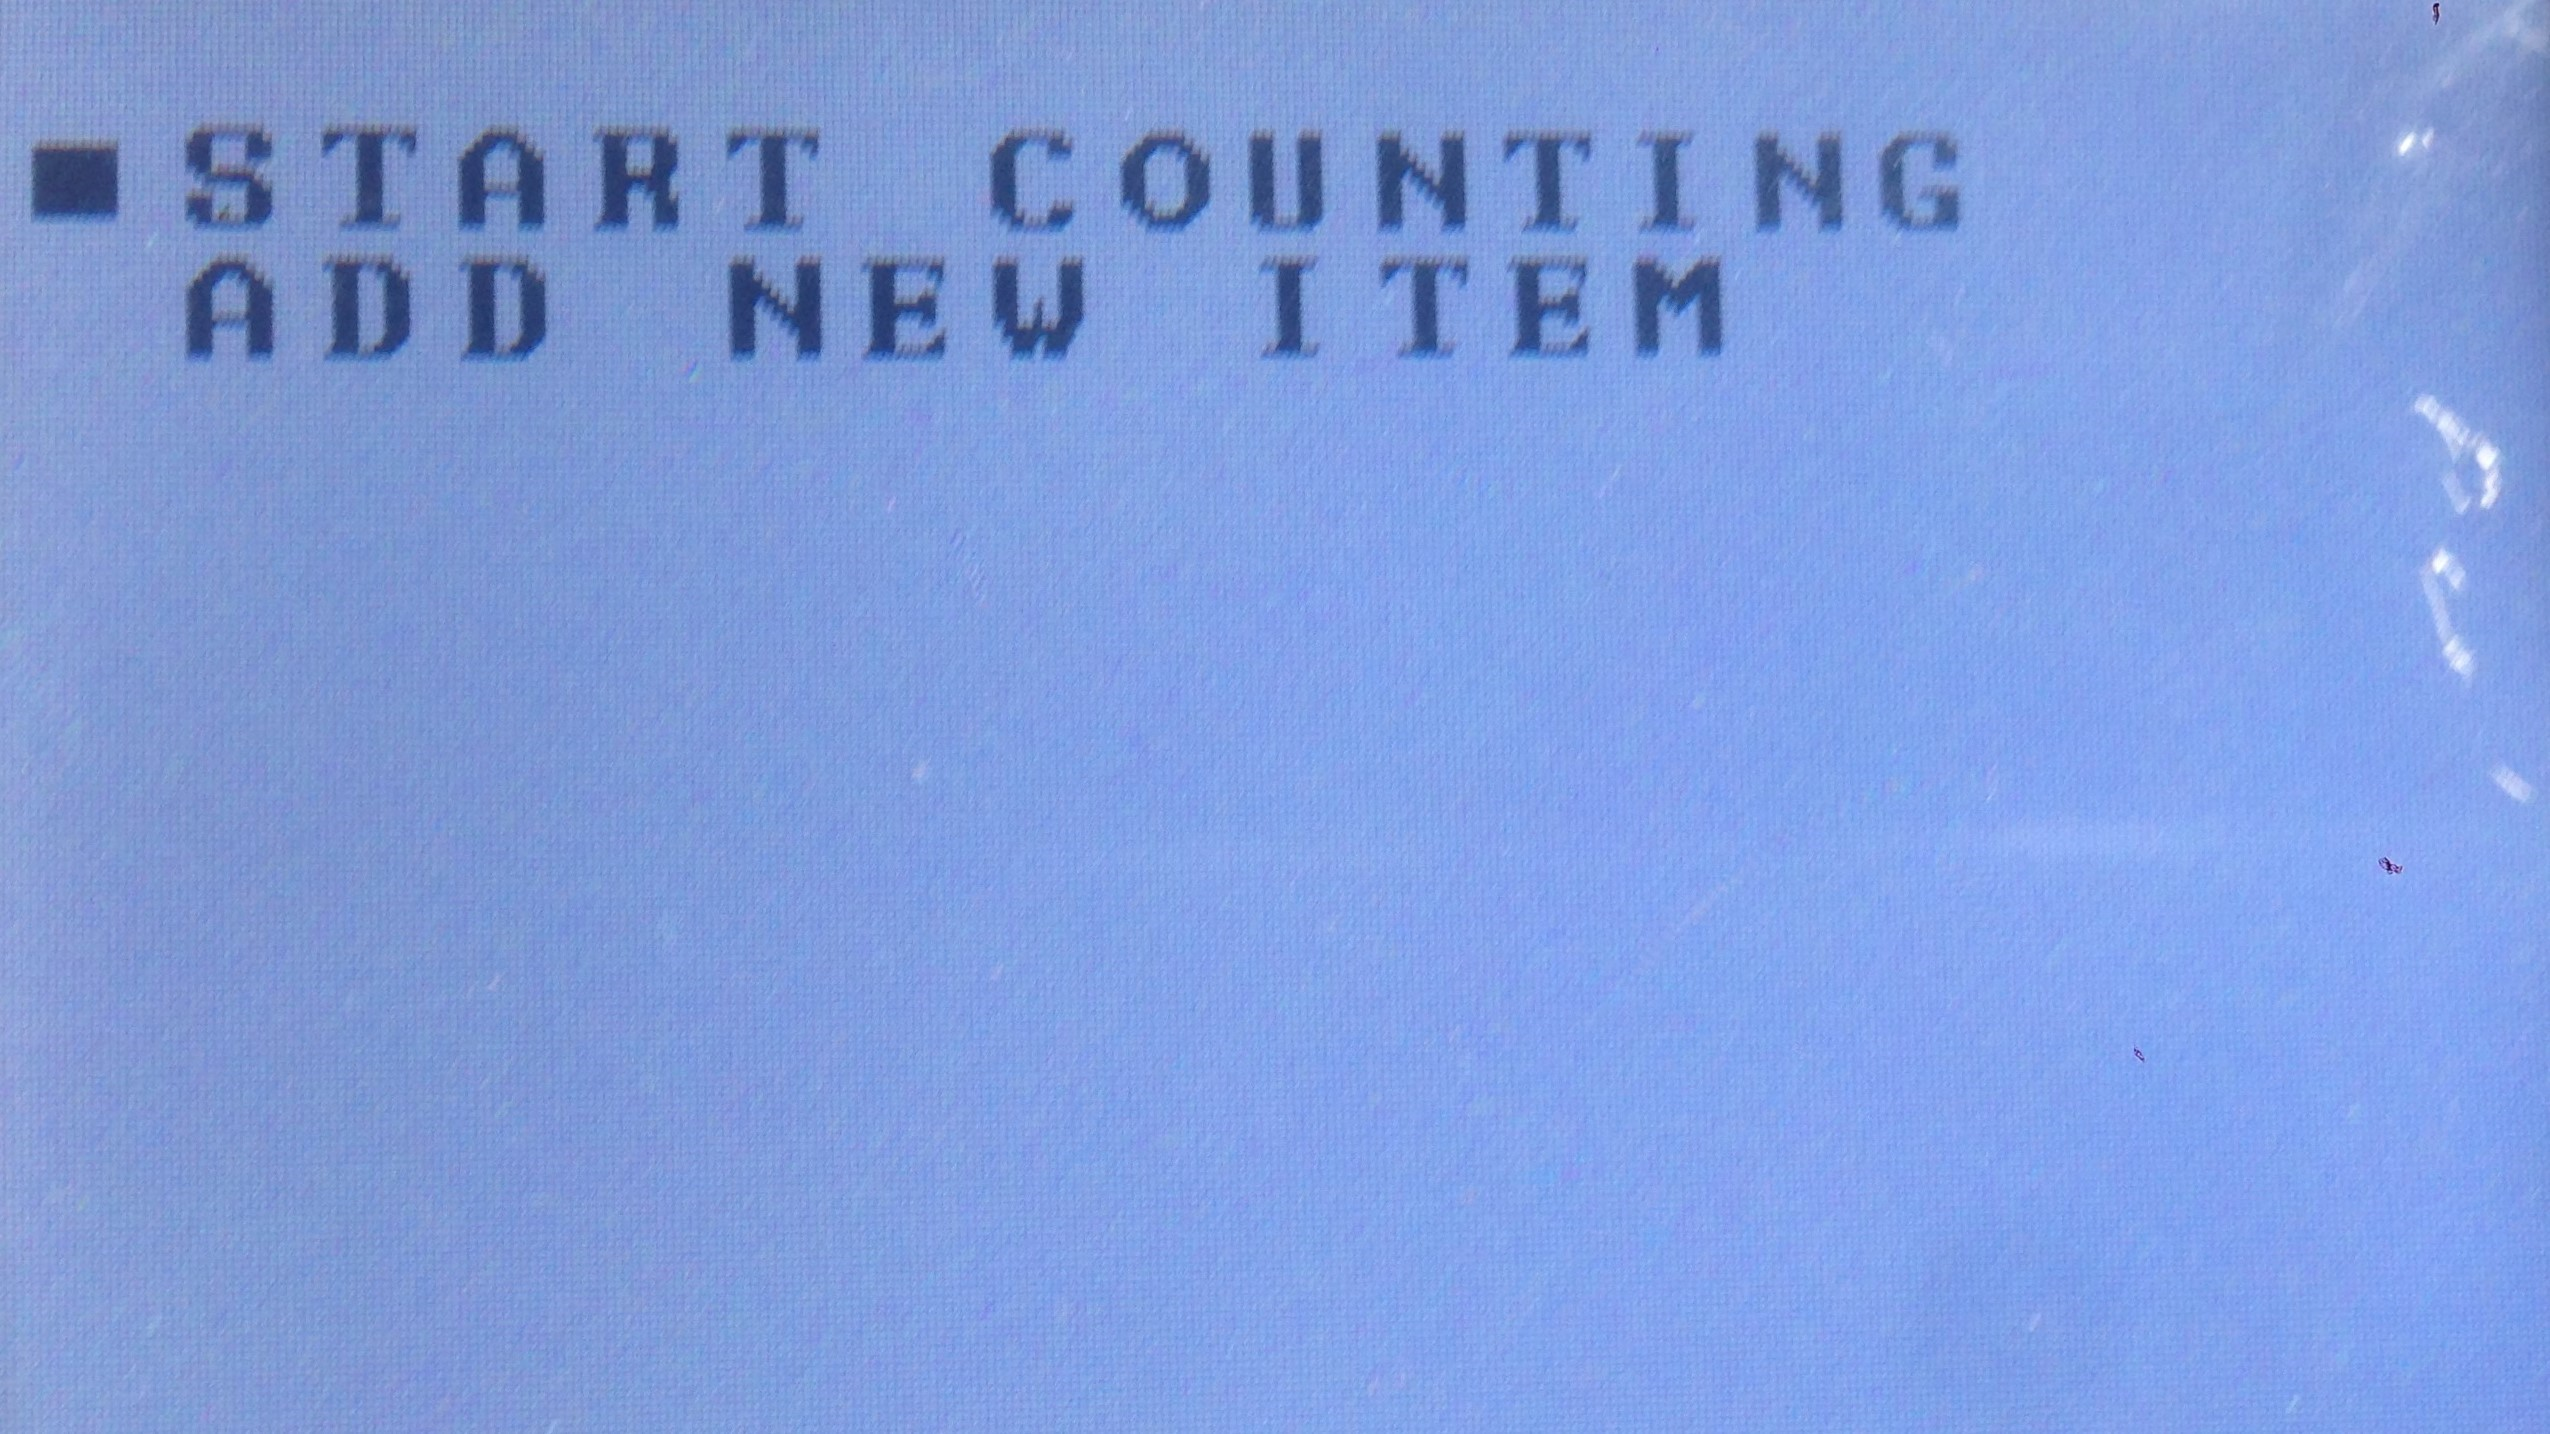
\includegraphics[width=.48\textwidth]{graphics/StartMenuScreen}\label{fig:StartMenuScreen}}
	\hfill
	\subfloat[The list of items to choose between when using the weight counter.]{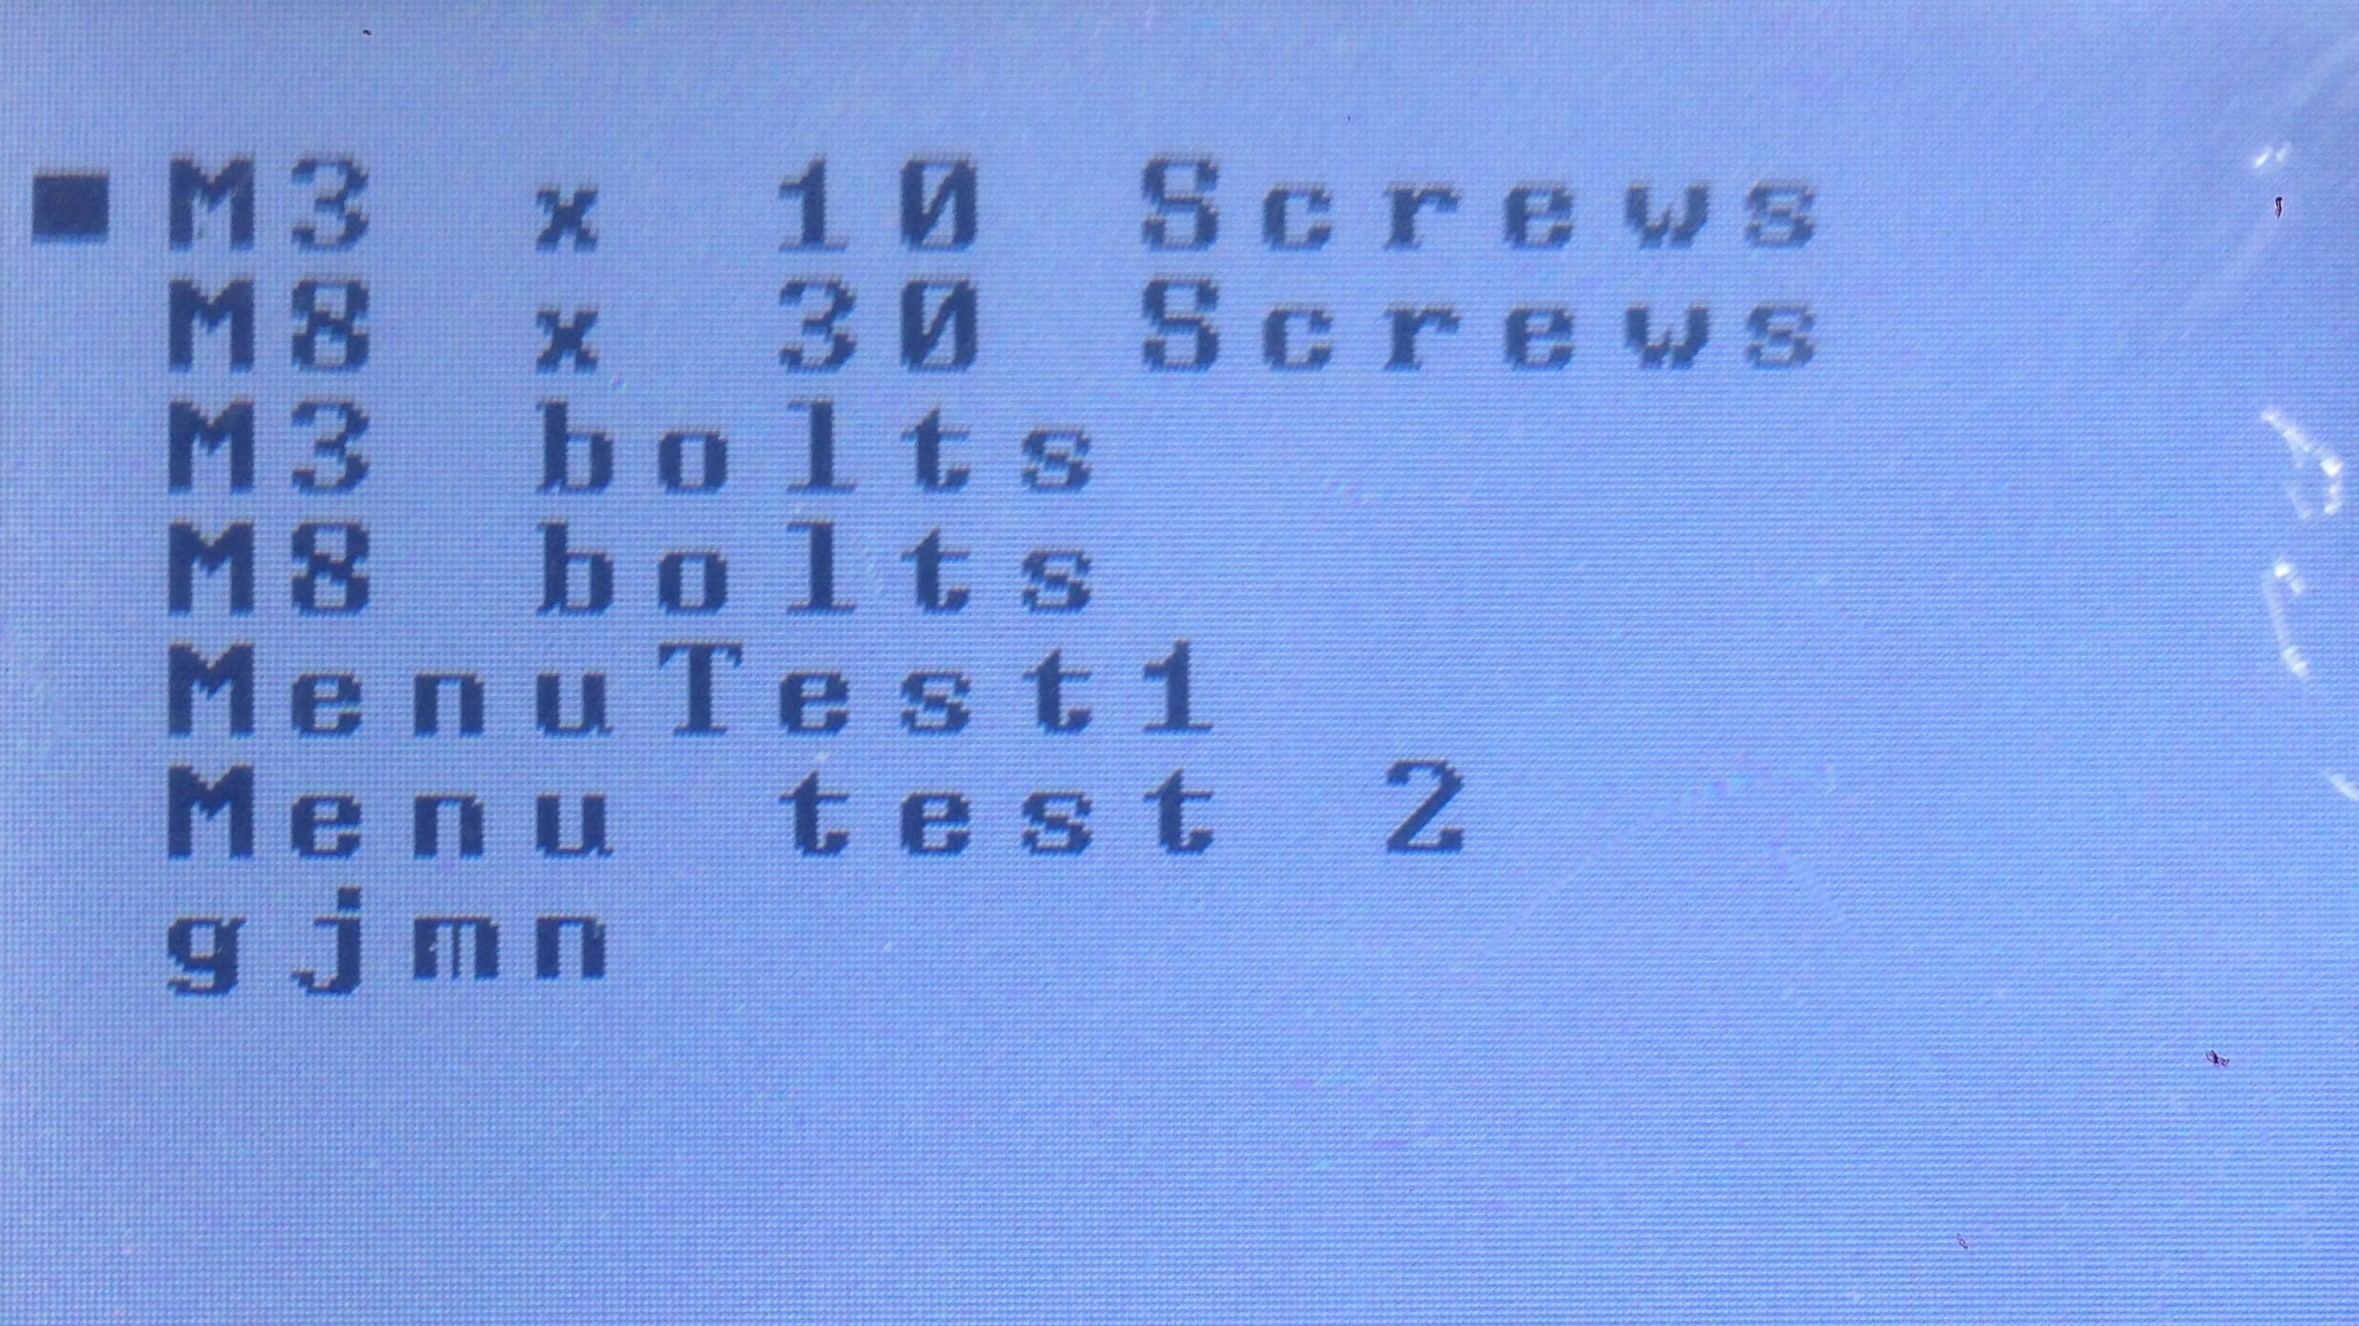
\includegraphics[width=.48\textwidth]{graphics/ListObjects}\label{fig:ListObjects}}
	\caption{Menu showing start menu and list of items menu.}	
\end{figure}


The black dot indicates the menu item which will be selected if the user presses the square key. If the user chooses start counting the output on the display can be seen in \cref{fig:ListObjects}. The display  will show as many menu items as there can fit in one column on the screen. If the chosen item will move outside the list then the whole list moves in the corresponding direction instead.

\begin{figure}[H]
	\centering
	\subfloat[Screen showing when the weight counter is selected and the item is selected.]{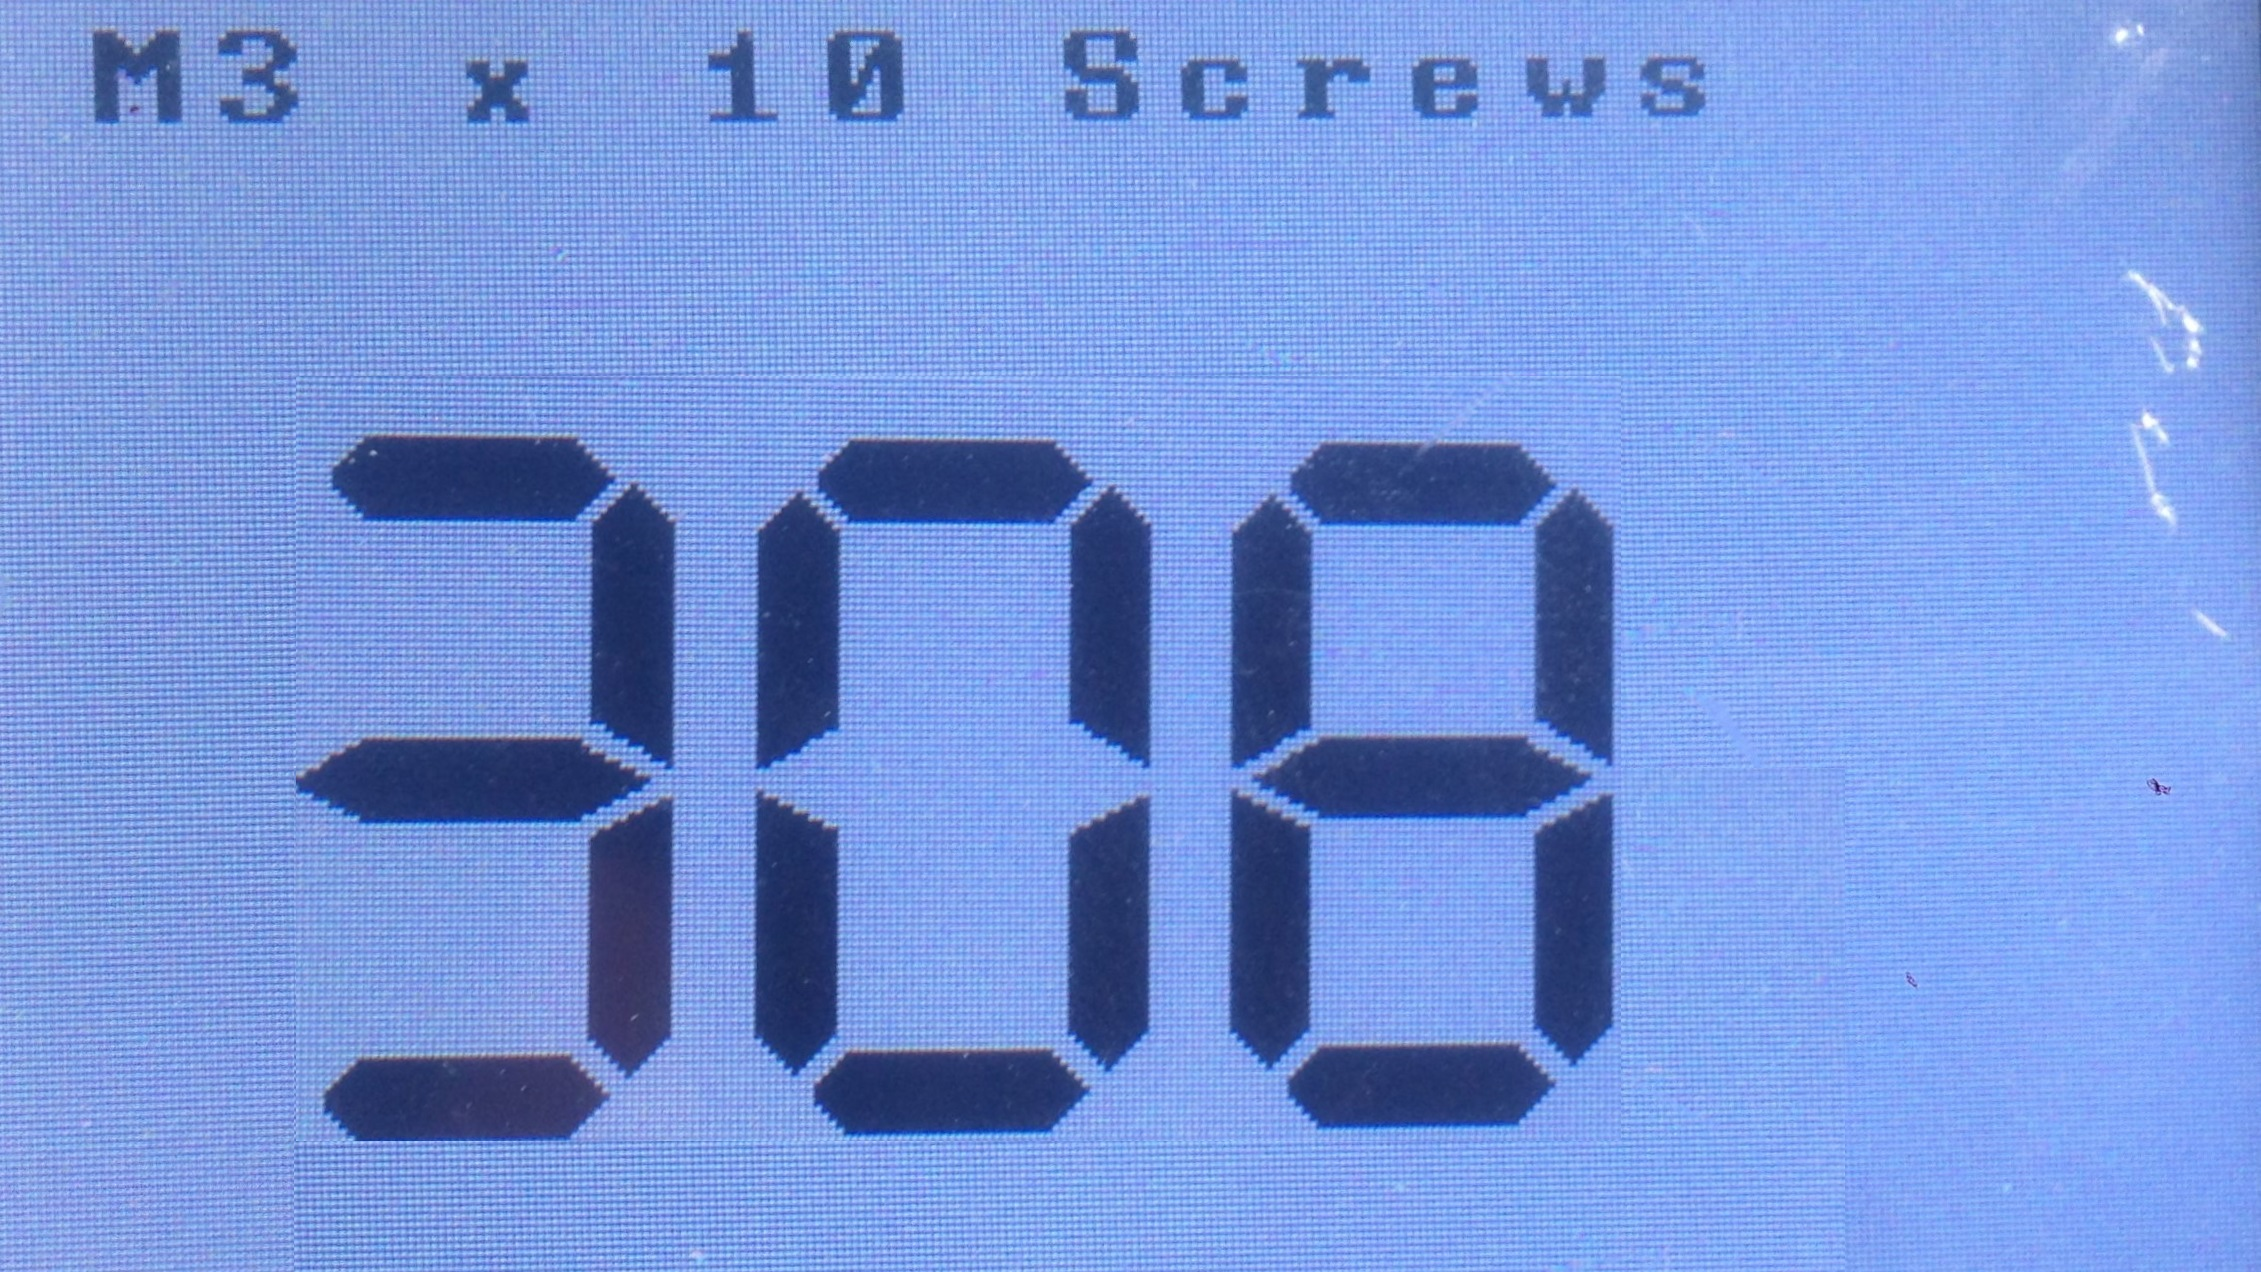
\includegraphics[width=.48\textwidth]{graphics/WeightCount}\label{fig:WeightCount}}
	\hfill
	\subfloat[The User can enter the name of a new item to be added. This item can be used with the weight counter.]{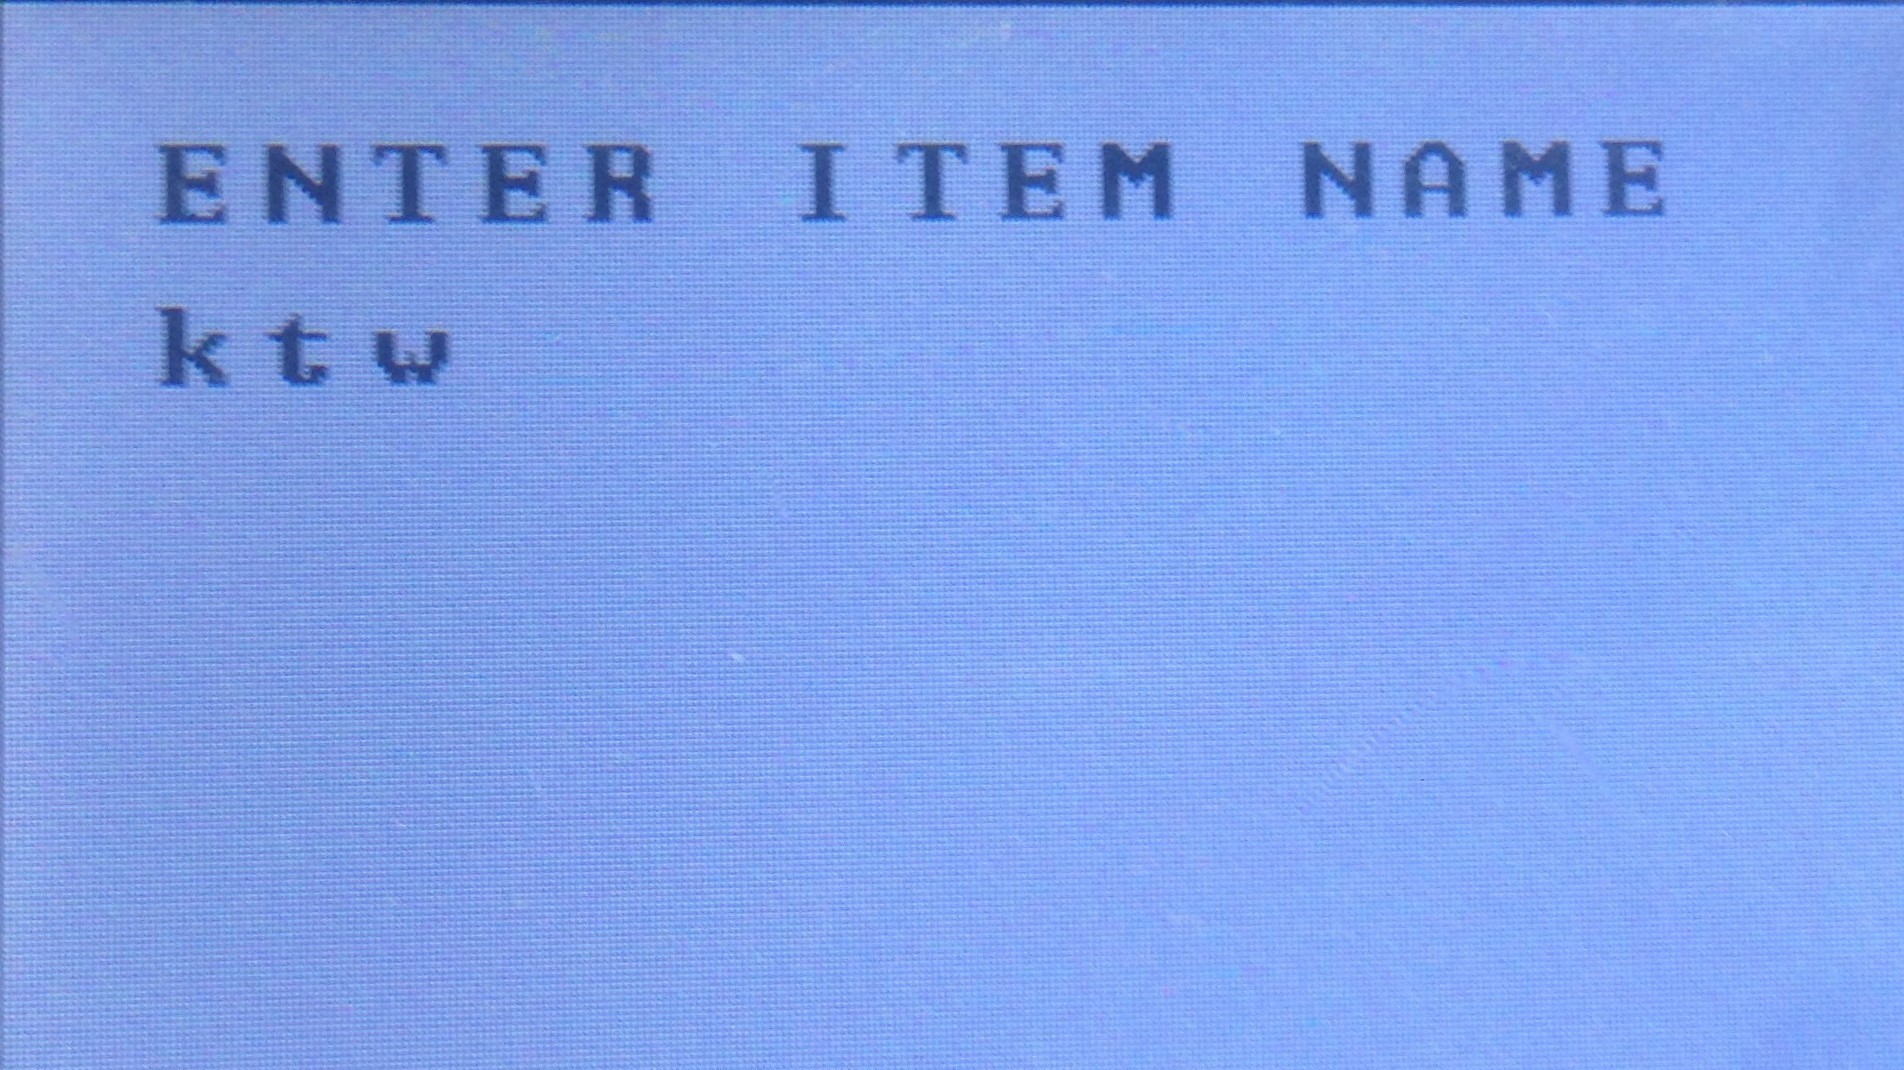
\includegraphics[width=.48\textwidth]{graphics/EnterName}\label{fig:EnterName}}
	\caption{Menu showing weight menu and new item name menu.}	
\end{figure}

When the item is selected by the user, the weight counter screen is shown see \cref{fig:WeightCount}. This is done by calling the \mintinline{c}{Counter} function. 
If the user selects add new item in \cref{fig:StartMenuScreen} the display will show a prompt for the user to enter the name for the new item, see \cref{fig:EnterName}.
The user can enter the name using a keypad. It is possible to delete already entered characters. When the user is finished inputting the name, the square button will proceed to the next part. The next part can be seen in \cref{fig:itemsOnScale}. The user is told to place a number of the items to be added to the weight counter.

\begin{figure}[H]
	\centering
	\subfloat[The user is told to place items on scale so an average weight of the item can be calculated.]{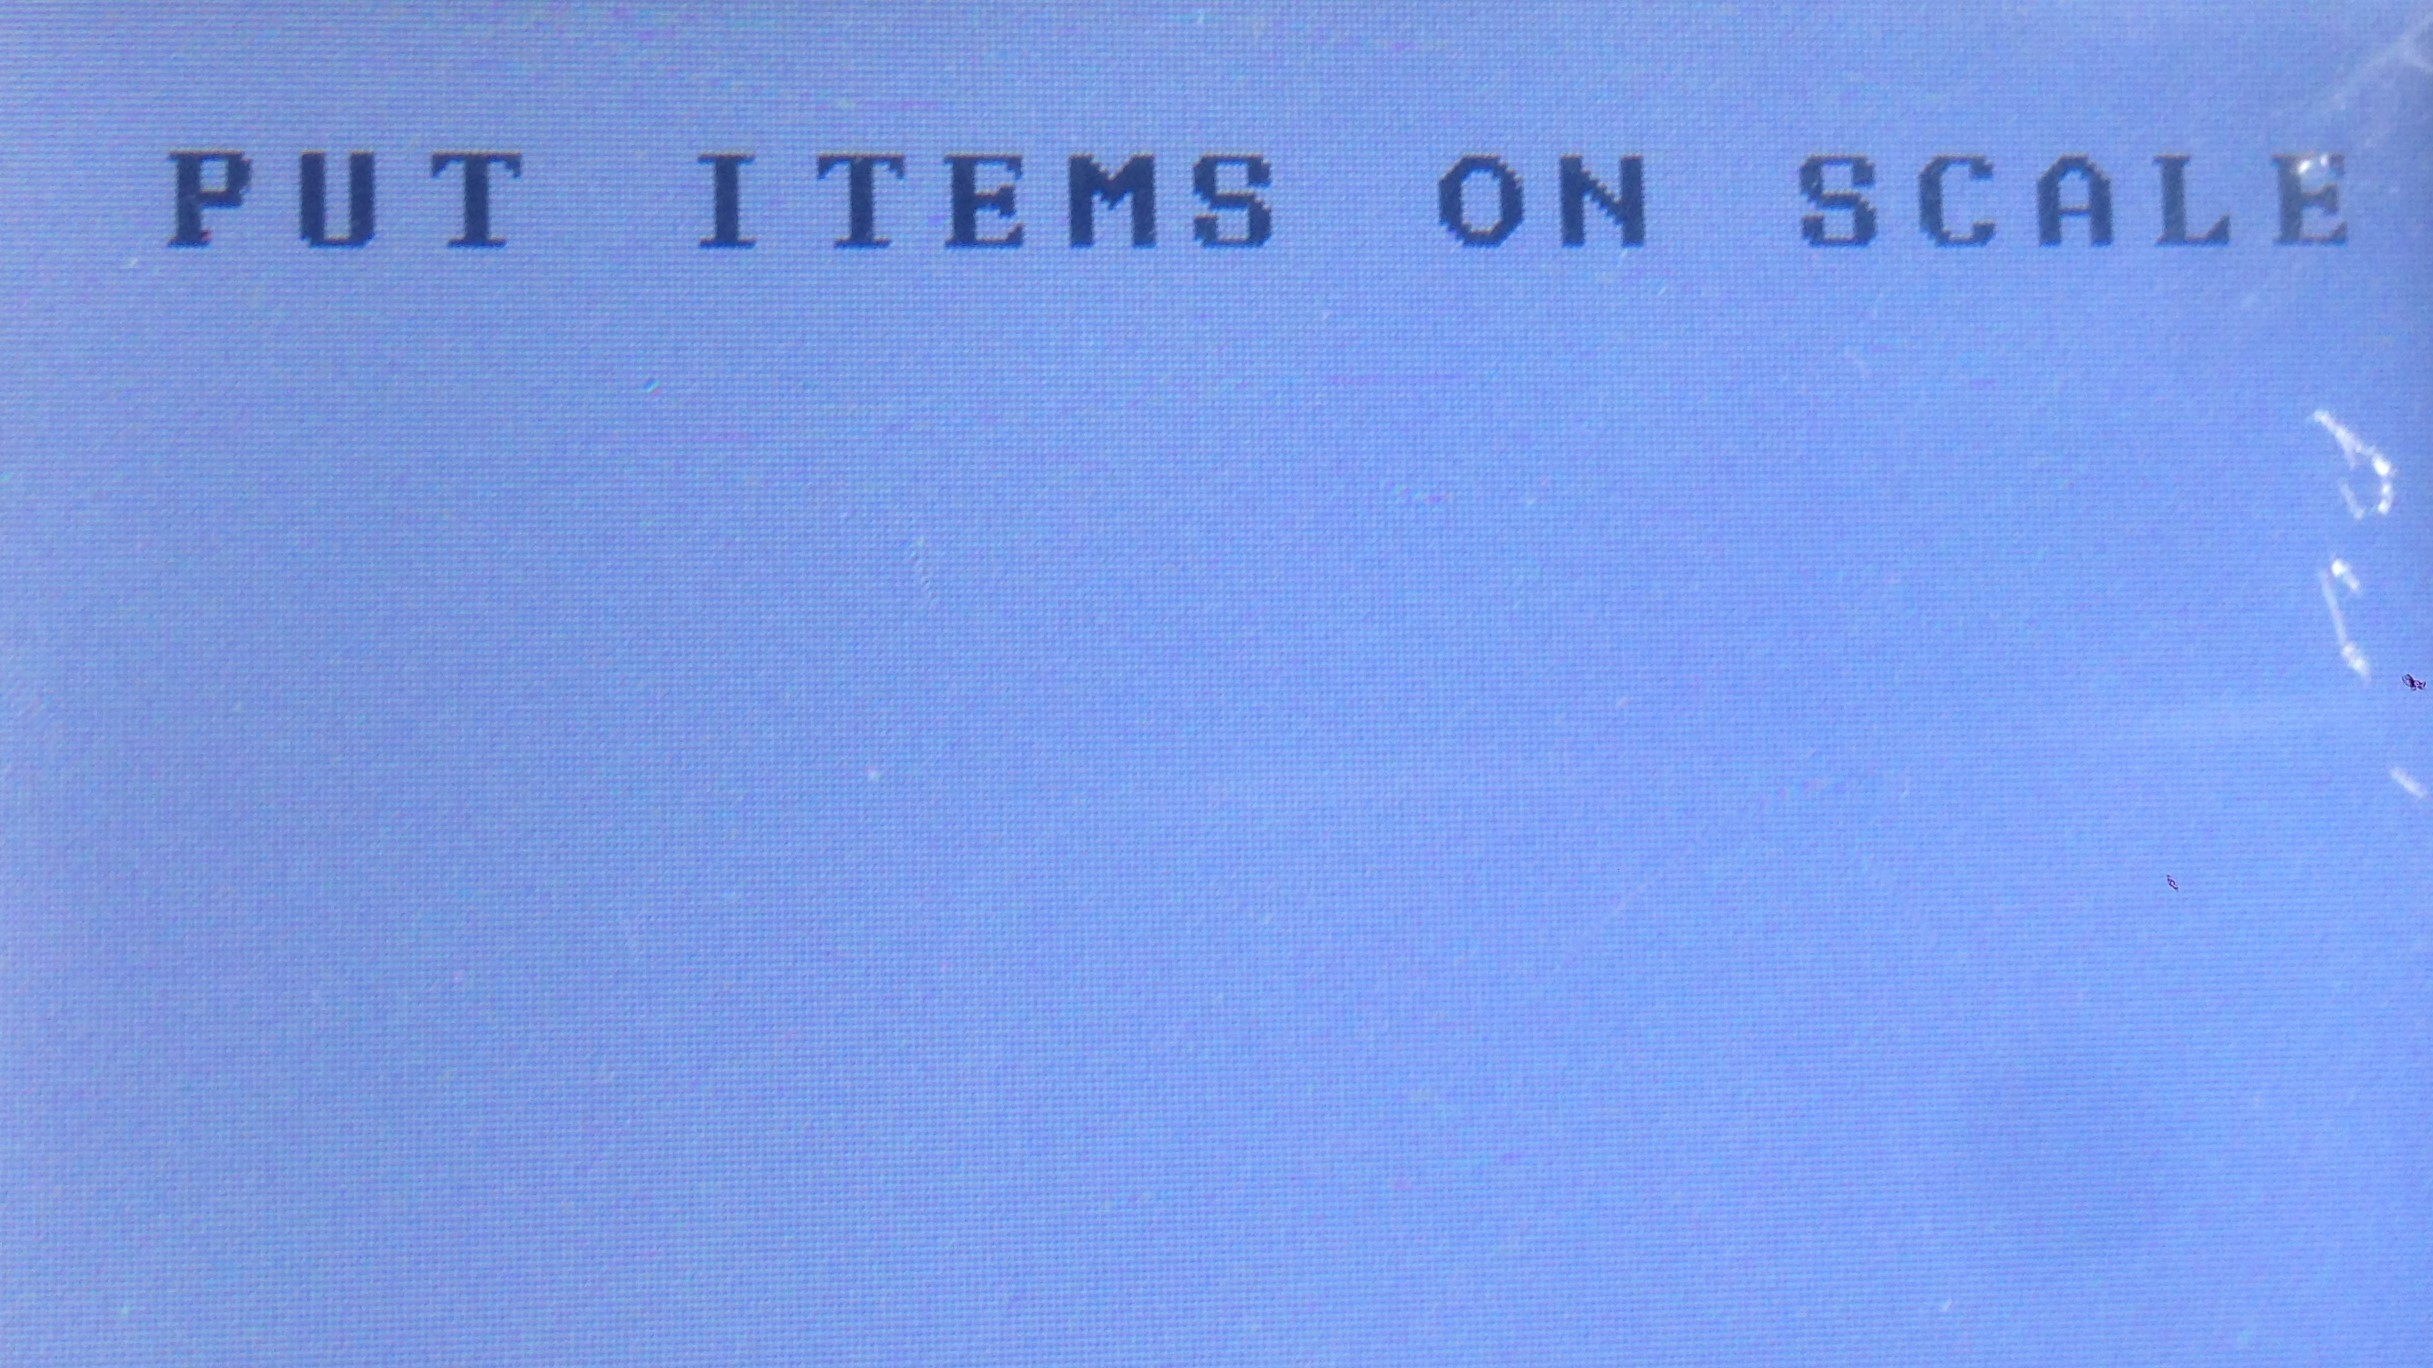
\includegraphics[width=.48\textwidth]{graphics/itemsOnScale}\label{fig:itemsOnScale}}
	\hfill
	\subfloat[The User can enter the name of a new item to be added. This item can be used with the weight counter.]{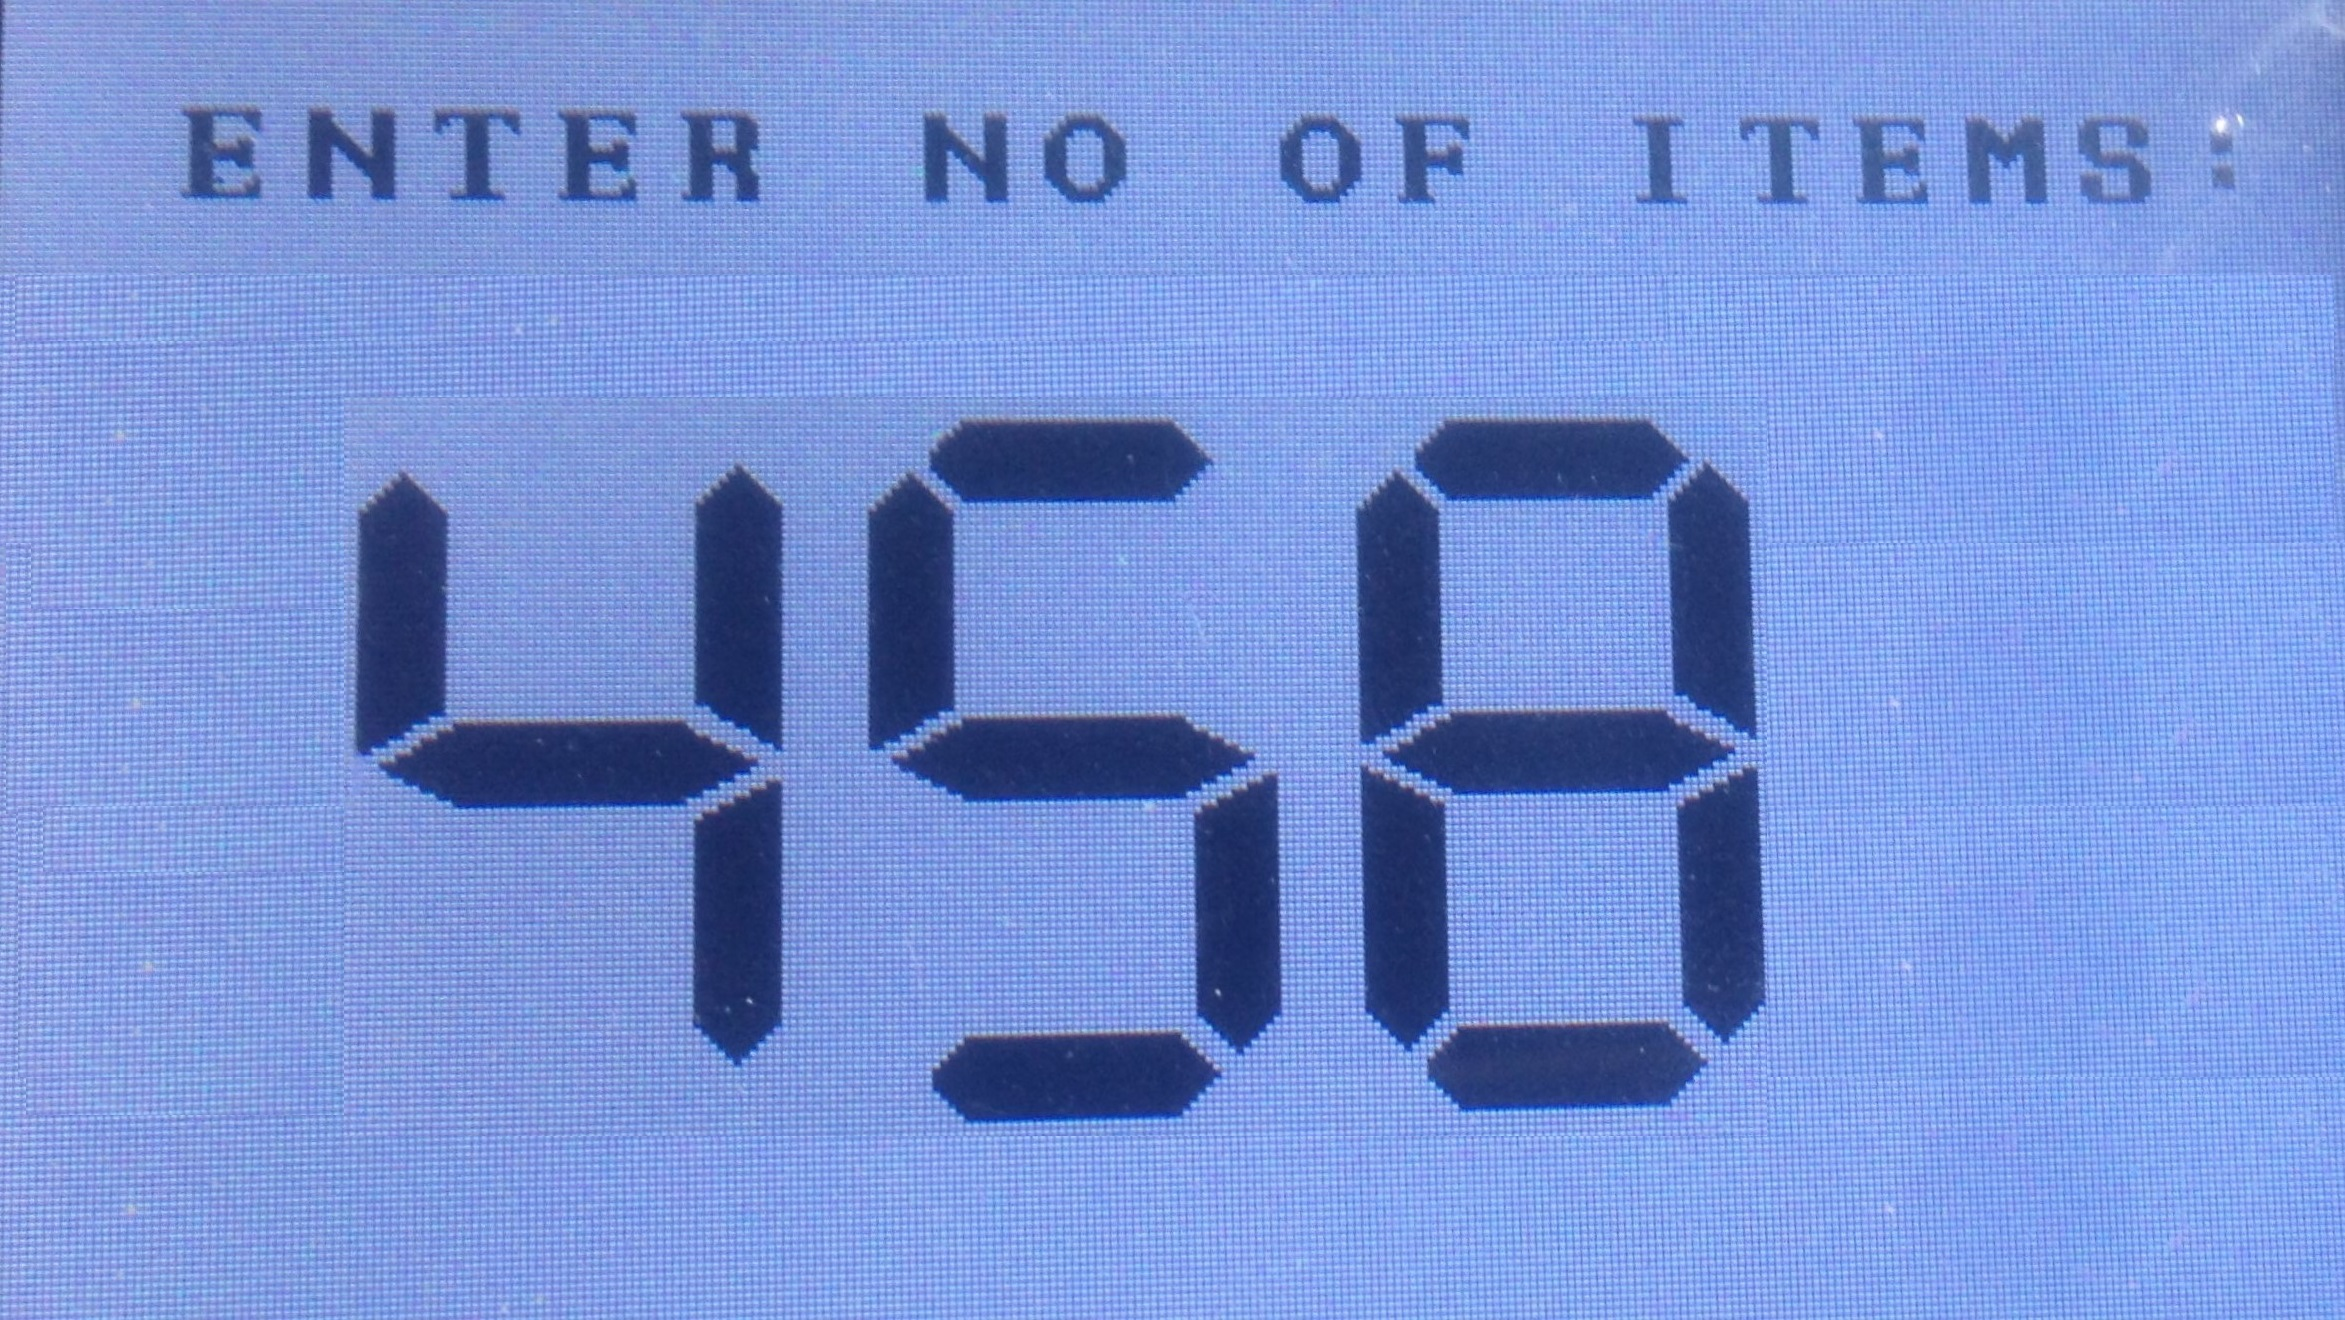
\includegraphics[width=.48\textwidth]{graphics/NoItems}\label{fig:NoItems}}
	\caption{Menu showing instruction to out items on scale menu and instruction to enter number of items menu.}	
\end{figure}

When the items are placed on the scale, the user continues to the next screen which can be seen on \cref{fig:NoItems}. The user enter how many items have been placed on the scale. When the amount has been entered, the name and average weight is stored permanently in memory even if the device is powered off.

This is done by using the eeprom feature of the ATMega2560. The eeprom is non volatile with $100\,000$ write cycles. The advantage of using eeprom compared to flash memory is that the program is placed in flash memory. Placing the data in flash would require part of it to only hold the data and not the program. The eeprom is currrently unused so it is simpler to implement. The other advantage is more write cycles for the eeprom than flash, $100\,000$ compared to $10\,000$. It is unlikely to use this many writes to non volatile memory in this application. Another advantage is the ability of eeprom to be accessed as bytes where flash can only be accessed as pages. Since the data being accessed is quite small, eeprom has the ability to only read or write the required data. The eeprom is implemented using the avr-libc library eeprom. \cite{EEPROM} The functions that are used with eeprom can be seen in \cref{lst:eeprom}. The \mintinline{c}{eeprom_update_block} saves the new name and \mintinline{c}{eeprom_update_float} saves the average value in eeprom. At the start up of the weight counter data is transferred from eeprom to RAM since it is slower to read data from eeprom than getting data from RAM. This is done by using the functions \mintinline{c}{eeprom_read_block} and \mintinline{c}{eeprom_read_float} for the name and average weight respectively. The block functions allows the transfer of a variable length of bytes. The type these functions take is void pointers which means the type of data is not used by the function allowing all types to be transferred.
\vspace{-10pt}
\begin{lstlisting}[caption={EEPROM functions.}, label={lst:eeprom}, language=C, directivestyle={\color{black}},
emph={int,char,double,float,unsigned},emphstyle={\color{blue}}]
void eeprom_update_block(const void * __src,void * __dst,size_t __n)
void eeprom_update_float(float * __p,float __value)
void eeprom_read_block(void * __dst,const void * __src,size_t __n)
float eeprom_read_float(const float * __p)
\end{lstlisting}
\vspace{10pt}

The eeprom has been tested by adding new entries to the weight counter with "ADD NEW ITEM". The item has been added along with the amount of items that were placed on the scale. After power up the added menu entry can still be found in the list under "START COUNTING".